\chapter{2-D Non-linear Weak Learner}
\label{sec:2dweaklearner}
%weak learner is no longer binary classifier
Although the multi-class classifier can be made from the combination of many binary classifiers with the voting rule, it requires the massive training on the whole set of binary classifiers. The multi-class weak learners should be simple and fast, such that the AdaBoost training can be finished in an appropriate time. An example of multi-class classifiers is the $k$ nearest neighbour classifier, which is easy to implement and fast running.

%difficult to find multi-class boundaries in 1D linear weak learner
\paragraph{More than One Dimension}
The Potsu weak learner is built on one single Gabor wavelet feature, so that the training data fed into the Potsu weak learner is the one-dimensional data. The classification can be quickly performed by using simple thresholding. However, in the case of multi-class, there are not only positive and negative, but more classes are available. To use simple thresholding technique in one-dimension is to separate the multi-class data with multiple thresholds. In other words, the multiple thresholds are to define the range of one-dimensional data with a certain class. However, the multiple thresholds in one-dimensional data may fail in finding the range of each class if some ranges are overlapped. Hence, for the multi-class case, the data in one-dimensional order is adverse for the classification. To improve the performance, the data must reside in the space which is more than one-dimension. In this section, the multi-class data resides in two-dimensional space.

%non-linear weak learner may appropriate for multi-class classification
\paragraph{Nonlinearity}
In general multi-class classification, if the features are well selected, the data from the same class will congregate into a cluster. If there are $k$ classes, it will be $k$ clusters. Every cluster should be well separated from each other as \mbox{Figure} \ref{fig:clusterperclass} shown. 
\begin{figure}[ht]
 \begin{center}
  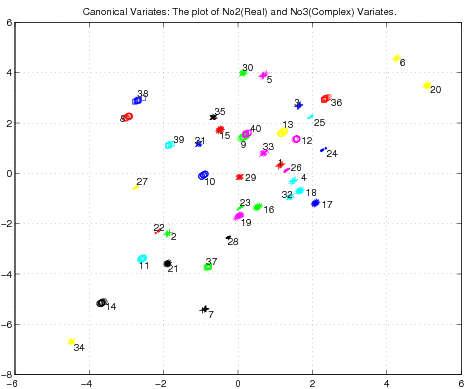
\includegraphics[width=0.66\columnwidth]{ch5/figures/Canonical_Variate_2_3.png}
  \caption{The example shows 10 face images for each of 40 different persons are formed into a cluster, and these clusters are well separated. }
\label{fig:clusterperclass}
 \end{center}
\end{figure} 
In \mbox{Figure} \ref{fig:clusterperclass}, there are ten examples in each class, and there are $40$ different classes. Every ten examples from the same class are formed into a tiny cluster, so that there are $40$ separated clusters. Linear discriminate approaches are expensive for being applied on these clusters , because this kind of approaches will at least be to define two linear discriminate criteria (one is upper bound and the other is lower bound) to constrain each cluster. However, non-linear classification methods such as the $k$-nearest neighbour classifiers are less expensive, because they do not use two lines to bound the cluster, but use distance and votes to define the criterion. Hence, non-linear classifiers are more appropriate to be adopted as weak learners in multi-class Gabor-Boosting. In the binary Gabor-Boosting classification, the final strong classifier is an non-linear classifier which is made with a linear combination of a group of linear classifiers with corresponding weights, \textit{i.e.}, importance. If the features are well chosen, the high-dimensional data is more likely resided in a linear manifold. However, those features which could express the linearity of data are difficult to select, so that the high-dimensional data mostly resided in an non-linear manifold \cite{Tenenbaum2000}. The binary Gabor-Boosting is to apply the non-linear classification technique on the high-dimensional data with non-linear structure. In multi-class Gabor-Boosting, not only the final classifier is non-linear, but also every weak learner inside the final classifier is non-linear. 

%weak classifier consists of 2 features - Gabor Feature Pair
\paragraph{Gabor Feature Pair}
Weak learners are trained based on one single Gabor wavelet feature. No matter linear or non-linear classification mechanism applied on the weak learner, the weak learner is still a linear classifier, because to classify one-dimensional data is equal to set a threshold on these data. In order to apply non-linear classification on the weak learner, the dimensionality of data must be more than one. Hence, a 2-D weak learner is defined, which consists of two Gabor wavelet features. In the thesis, the two Gabor wavelet features are called \textbf{Gabor Feature Pair} or \textbf{GFP}. By using Gabor feature pair, the 2-D weak learners form a two-dimensional feature space.

%knn is applied to find the optimal boundary to minimise the error rate of weak classifier.
\paragraph{$k$-NN}
The classification mechanism on the 2-D weak learners with GFP should be non-linear, so the $k$ nearest neighbour ($k$-NN) classifier is chosen. 

The choice of $k$ is depend upon the data.  Generally, larger values of $k$ reduce the effect of noise on the classification, but make boundaries between classes more vague. A good $k$ can be selected by heuristic techniques. In the 2-D weak learner, the choice of $k$ is done by assuming $k$ in a set $\{1,3,4,\ldots,32\}$, build a $k$-NN classifier with the corresponding number in the set, and find the optimal $k$ is the $k$-NN with the minimum training error.

%advantage for GFP

\section{Mutual Information on Gabor Feature Pair}
%massive pair
If the number of available features is $n$, the number of available GFPs will be $n(n-1)/2$. In the \mbox{XM2VTS} database, each example is in order of $30,240$ features after the \textbf{Scaling} pre-selection scheme. All $30,240$ features are used to make GFPs, and there are $30240\times (30240-1)/2=457,213,680$ GFPs for AdaBoost to select. To select the most significant GFPs from these $457,213,680$, the whole training will be extremely time costly. Therefore, it is necessary to filter some GFPs, then put the rest GFPs into AdaBoost training to select pairs with the lowest mutual information. In this thesis, \textit{Mutual Information} \cite{Peng2005,Shan2005} is evaluated within a GFP. Based on the value of Mutual information, some pairs are rejected, but some are accepted.

\subsection{Mutual Information}
In information theory, mutual information between two random variables is a quantity that measures the mutual dependence of the two variables. If one variable random is derived from another variable, the mutual information between the two variables will be large. If two variables are independent with each other, the mutual information between them will be zero. Mutual information measures the dependence between two variables. In telecommunication, since signal channel is limited, two variables with higher mutual information lead to information redundancy which is the amount of wasted ``space'' used to transmit certain data. In general, mutual information is required to be as small as possible to avoid information redundancy. 

The concept of mutual information is very close to another concept \textit{correlation} in statistics. The correlation is another frequently used quantity to measure the dependence. It is now well understood \cite{Li1990} that mutual information measures the general dependence, while the correlation measures the linear dependence. Hence, mutual information is a better quantity than correlation to measure the dependence.

Formally, the mutual information $I(X;Y)$ of two discrete random variables $X$ and $Y$ can be defined as
\begin{eqnarray}
 I(X;Y) = H(X) - H(X|Y) \nonumber \\
= H(Y) - H(Y|X) \nonumber \\ 
 = H(X) + H(Y) - H(X,Y) 
\end{eqnarray}
where $H(X)$ and $H(Y)$ are the entropies of variable $X$ and variable $Y$, $H(X|Y)$ and $H(Y|X)$ are the conditional entropies, and $H(X,Y)$ is the joint entropy of $X$ and $Y$. The entropy $H(X)$ is a measure of the uncertainty associated with a random variable $X$. It describes how much the information contained in a message. The entropy is the minimum message length necessary to communicate information. In communication, a random variable $X$ is required to be as uncertain as possible, otherwise the variable $X$ always describe a certain thing, which is unvaried and waste of signal channel. For a discrete random variable $X$ that can take on possible values $\{x_{1},\ldots,x_{n}\}$, the entropy $H(X)$ is defined as 
\begin{equation}
   H(X) =  - {\sum_{i=1}^np(x_i)\log_2 p(x_i)} 
\end{equation}
where $p(x_i)$ represents the marginal probability distribution of $X$.

The entropy $H(X|Y)$ is a measure of how $Y$ does not influence on $X$. The definition of $H(X|Y)$ is that, the amount of uncertainty remaining about $X$ after $Y$ is known. The formula $H(X) - H(X|Y)$  can be explained that the amount of uncertainty in $X$, minus the amount of uncertainty in $X$ which remains after $Y$ is known. The formula is equivalent to the amount of uncertainty in $X$ which is removed by knowing $Y$. In general, it confirms the intuitive meaning of mutual information as the amount of information that knowing either variable provides about the other.

\subsection{Mutual Information on GFP}
A Gabor feature pair contains two Gabor wavelet features $j_1$ and $j_2$. A Gabor feature pair is expressed as $\{j_{1},j_{2}\}$. The mutual information on the Gabor feature pair is $I(j_1;j_2)$, which measures the dependence between the feature $j_1$ and the feature $j_2$. The dependence between features displays redundancy and relevance of these two features. From the measurement of one feature, it is possible to predict the measurement of another feature if the mutual information is high. A pair which has lower mutual information is appropriate to feed into the 2-D weak learner.

The pre-selection on GFPs is based on thresholding mutual information. A threshold is set to accept the pair whose mutual information is less than the threshold, but to rejects other pairs whose mutual information are equal or more than the threshold. The threshold is an arbitrary quantity, which is measured by the accept rate and the distribution of mutual information on the whole set of pairs.

\subsection{Mutual Information Estimation}
The estimation of mutual information is followed by the implementation of \cite{Fleuret2004} which is to select fast binary features with Conditional Mutual Information. The estimation of the entropy, mutual information can be done by summing and subtracting estimation of entropies of two features $j_1$ and $j_2$. Each feature $j$ has $n$ possible values $\{j^{(1)},\ldots,j^{(n)}\}$. The mutual information on a Gabor feature pair $\{j_{1},j_{2}\}$ is
\begin{equation}
 I(j_1;j_2) = H(j_1) + H(j_2) - H(j_1,j_2)
\end{equation}
The entropy of a feature $j$ is
\begin{equation}
 H(j) = - {\sum_{i=1}^np(j^{(i)})\log p(j^{(i)})}
\end{equation}
A joint entropy of two features $j_1$ and $j_2$ is
\begin{equation}
 H(j_1,j_2) = -{\sum_{i=1}^n \sum_{i=1}^n  p(j_1^{(i)}, j_2^{(i)})    \log p(j_1^{(i)},j_2^{(i)}) }
\end{equation}
The estimation of mutual information is require to estimate the probability distribution $p(j)$ and the joint probability distribution $p(j_1,j_2)$. 

To estimate the probability distribution on discrete data, there are two ways to do the estimation. One way is to parameterise a probability density function (pdf) on the training data. The parameters of density function are obtained from analysing the training data. However, it requires a statistic model before the parameterisation. If the model is not appropriate for the training data, a false density function will be made, which leads to wrong probability at the end. In most of cases, the training data is assumed to be a single Gaussian distribution. Nevertheless, if the training data resides in a multiple mix Gaussian distribution, the establishment of building pdf is failed. In addition, the parameterisation is a very time-consuming process. 

Another way is to use \textit{Histogram search} to calculate the corresponding probability. In histogram search, all possible observations of the feature $j$ are fall into various disjoint categories, which is more called as \textbf{bins}. A bin represents a range of observations. For example, the observations of a feature $j$ is in a range of $[0\quad 1]$, a bin can be $[0.1\quad 0.2]$. It is set that $n$ be the total number of observations and $k$ be the total number of bins. Each observation of a feature $j$ must be fell into a bin, and the observation of a feature is represented by the corresponding bin. Hence, the probability of a particular observation of a feature $j$ is represented by the probability of corresponding bin. The probability of bin can be computed by 
\begin{equation}
p(\mathrm{BIN}) = \frac{k}{n}
\end{equation}
The probability distribution of a feature $j$ is the collection of the probabilities of all bins in the histogram. To locate which bin for a particular observation is, the \textit{Lookup Table} \cite{wiki:LUT} technique is used.

In this thesis, the probability distribution is estimated by the histogram search, because it is fast and easy to implement. If the model selection is valid on building pdf, the probability distribution is more accurate. However, because it is pre-selection on massive pairs, the speed is the main concern, and the accuracy is not so important.

The probability distribution of one feature is described above, however the joint probability distribution of two features is more sophisticated. There are two features $j_1$ and $j_2$, and the observations on each feature form a histogram. Each histogram is categorised into number of bins, such as $k$ bins. When both features $j_1$ and $j_1$ are given particular observations, two observations are fell into two bins. The joint probability $p(j_1^{(i)},j_2^{(i)})$ is the probability of two corresponding bins by counting number of observations when two bins are satisfied. The computation of joint probability is more expensive, because it actually categorises the observations into $k^2$ bins, and calculates the probability of each bin. 


\section{Results}
Computing mutual information on about 450 million pairs is extremely time consuming, such that Grid computing technology has been adopted to finish the huge amount of computation in a short time. The detail of technical implementations of how to calculate mutual information on these pairs by Grid computing is given in \mbox{Chapter} \ref{sec:gridcomputing}.

After the computation, there are $457,213,680$ mutual information obtained. The Gabor feature pairs with the lowest mutual information are expected to be acquired, because lower mutual information means more independent between two features in a pair. The lowest mutual information is $0.275347$, and there are $27,045$ pairs have the lowest one. A very interested phenomenon is found among these $27,045$ pairs, which is every pair contains a same feature $j(34,8, -1, 1)$ in the form of $j(x,y,\nu,\mu)$. These pairs which are constructed by $j(34,8, -1, 1)$ and all other features, have the lowest mutual information. The second lowest mutual information is $0.292102$, and there are $27,095$ pairs have the same mutual information. These pairs also contain a same feature $j(34,7, -1, 1)$. There are $45$ lowest mutual information investigated. With each lowest mutual information, there are many pairs share the same mutual information. Also these pairs contain one same feature for each lowest mutual information. Since each lowest mutual information reveal one same feature, the 45 lowest mutual information reveals $45$ features. These 45 features are projected on a mean face image as shown in \mbox{Figure} \ref{fig:mutinffeatures}.
\begin{figure}[ht]
 \begin{center}
  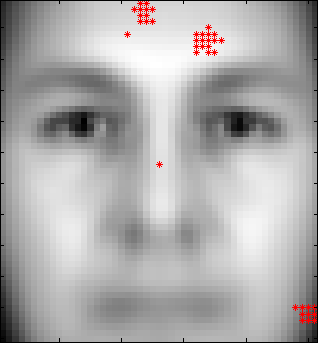
\includegraphics[scale=0.25]{ch5/figures/XM2VTS_mutinf.png}
  \caption{The 45 features with the lowest mutual information}
  \label{fig:mutinffeatures}
 \end{center}
\end{figure} 
All $45$ features are with the smallest spatial frequency $\nu=-1$. These 45 features form three clusters on face. Two clusters are on the forehead, and one cluster is on the left bottom. The first ten features are shown in \mbox{Figure} \ref{fig:mutinf10features}.
\begin{figure}[ht]
 \begin{center}
  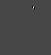
\includegraphics[width=\columnwidth/11]{ch5/figures/mutinf_01.png}
  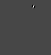
\includegraphics[width=\columnwidth/11]{ch5/figures/mutinf_02.png}
  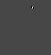
\includegraphics[width=\columnwidth/11]{ch5/figures/mutinf_03.png}
  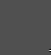
\includegraphics[width=\columnwidth/11]{ch5/figures/mutinf_04.png}
  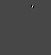
\includegraphics[width=\columnwidth/11]{ch5/figures/mutinf_05.png}
  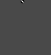
\includegraphics[width=\columnwidth/11]{ch5/figures/mutinf_06.png}
  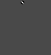
\includegraphics[width=\columnwidth/11]{ch5/figures/mutinf_07.png}
  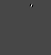
\includegraphics[width=\columnwidth/11]{ch5/figures/mutinf_08.png}
  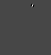
\includegraphics[width=\columnwidth/11]{ch5/figures/mutinf_09.png}
  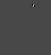
\includegraphics[width=\columnwidth/11]{ch5/figures/mutinf_10.png}\\
  \caption{The first ten features obtained from the mutual information computation.}
  \label{fig:mutinf10features}
 \end{center}
\end{figure} 
It is clear that these features are highly correlated so that they are not appropriate for further classification. However, the clusters may indicate some important regions on faces.